\section{模型}

\subsection{问题描述}
首先基于统计数据,
然后建立交通网络的模型,根据模型列出对应的VSP问题方程并求解,以便之后优化问题的求解和模拟,
使用SimPy包对不同结果进行模拟。

\subsection{单服务台负指数分布排队系统}
在串行的k个车站中,每个车站的服务时间相互独立,服务时间服从参数为 $k \mu$ 的负指数分布,称总服务时间服从 $k$ 阶爱尔郎分布。
爱尔朗分布族提供更为广泛的模型类,比指数分布有更大的适应性。事实上,当 k = 1 时, 爱尔朗分布化为负指数分布,进一步可推导出对于单个车站
$k=1$ 的情况下到达人数近似服从泊松分布,由于泊松分布的无记忆性\cite{gll},可以更好的描述一个排队系统。
\begin{figure}[htbp!]
    \centering
    \subfigure[k=1的爱尔郎分布\label{fig31:sub1}]{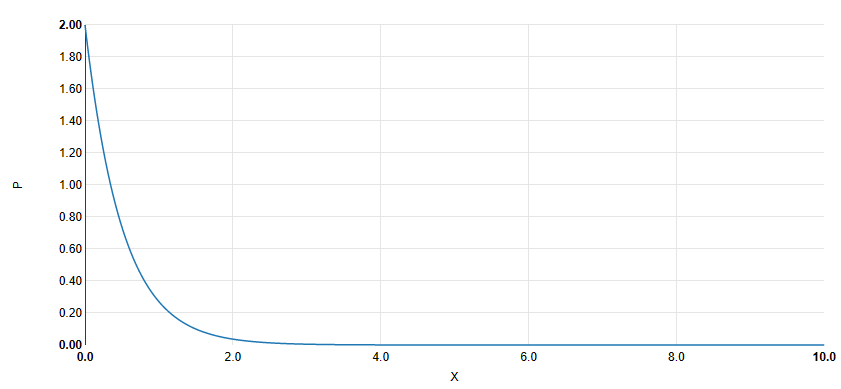
\includegraphics[width=0.4\textwidth]{figs/chap03/elarng.png}}
    \subfigure[泊松分布\label{fig31:sub2}]{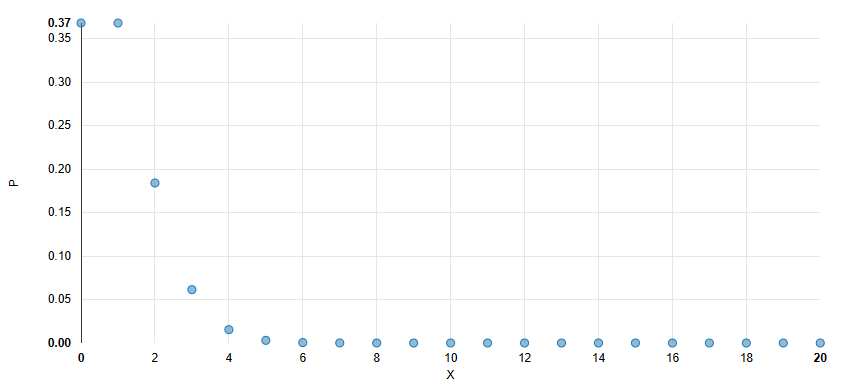
\includegraphics[width=0.4\textwidth]{figs/chap03/possion.png}}
    \caption{两种分布对比图}
    \label{dis1}
\end{figure}


前文给出了单服务台负指数分布排队系统(M/M/1/ $\infty $ / $\infty $)的基本方程~\ref{fomula1}~和状态图~\ref{fig21}~,由图图~\ref{fig21}~
可知,状态 $0$ 转移到状态 $1$ 的转移率为 $\lambda P_0$ ,状态 $1$ 转移到状态 $0$ 的转移率为 $\mu P_1$。由排队系统生灭状态的平衡性质可知,对于状态0必须满足如下方程:
$$\lambda P_0 = \mu P_1$$
对于任意的 $n \ge 1$ 的状态,都可以得到式~\ref{fomula1}~中的方程,求解~\ref{fomula1}~得:
$$P_1 = (\lambda / \mu)P_0$$
易证:
$$P_2 = \left(\lambda / \mu \right)^2 P_0$$
$$……$$
$$P_n = \left(\lambda / \mu \right)^n P_0$$
令 $\rho = \frac{\lambda}{\mu} < 1$,由概率的性质
$$\sum_{n=0}^{\infty}p_n = 1$$ 可以得到站台中乘客数为n的概率 $$P_n = (1-\rho)\rho^n, n \le 1, \rho < 1$$
其中 $\rho$ 代表系统的平均服务率,它刻画了服务机构的繁忙程度;所以又称服务机构的利用率。

由此可以得到一个平均到达率为 $\lambda$,平均服务率 $\mu$ 的排队系统的几个主要指标:

(1)乘客到达后不能及时得到服务需要等待的概率(系统服务强度):
$$P_w = \frac{\lambda}{\mu}$$

(2)系统空闲的概率:
$$P_0 = 1-\frac{\lambda}{\mu}$$

(3)系统中平均乘客长度(队长的期望值)
$$L_s = \frac{\lambda}{\mu - \lambda}$$

(4)在队列中等待的平均顾客数(队列长期望值)
$$L_q = L_s - \rho = \frac{\rho \lambda}{\mu - \lambda}$$

(5)在系统中顾客逗留时间的期望值
$$W_s = E[W] = \frac{1}{\mu - \lambda}$$

(6)队列中顾客等待时间的期望值
$$W_q = W_s - \frac{1}{\mu} = \frac{\rho}{\mu - \lambda}$$


解决排队问题首先要根据原始资料作出乘客到达间隔和服务时间的经验分布,根据以往经验,校园公交车站客流呈周期性变化,
选择文德楼北上行线车站实地统计,该车站位于校门、宿舍楼、主教学楼连接处的枢纽位置,客流量较有代表性,采样地点如图~\ref{fig31}~。
\begin{figure}[htbp!]
    \centering
    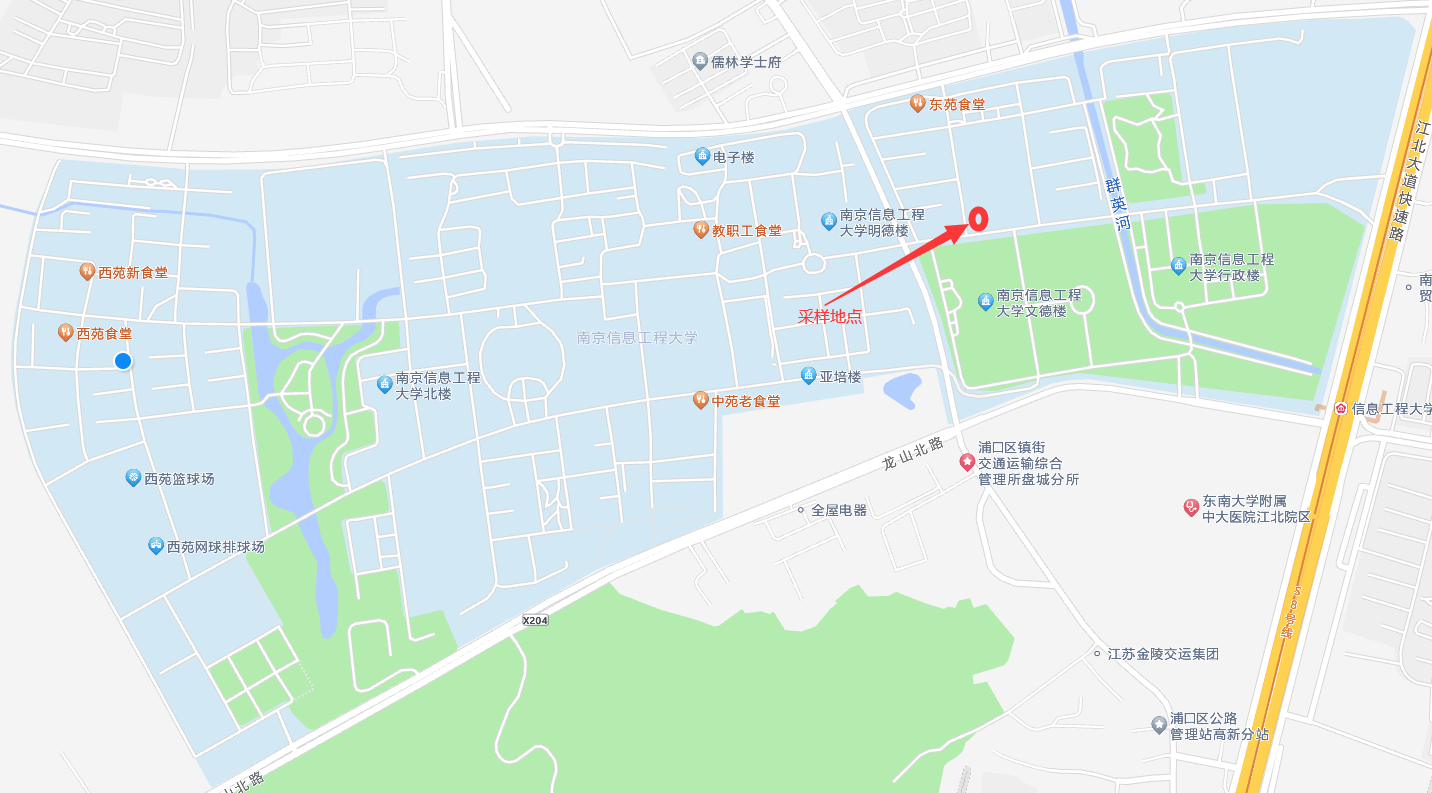
\includegraphics[width=0.80\textwidth]{figs/chap03/map.png}
    \caption{采样地点}
    \label{fig31}
\end{figure}

以大约两节课的时间(两小时)为一个周期,5分钟为间隔进行采样,所得的一个周期内的客流分布如表~\ref{table_1}~所示。
\begin{table}[htbp!]
    \centering
    \caption{车站乘客到达人数分布表}\label{table_1}
    
    \begin{tabular}{cccc}
    \whline 
    时间段 & 到达人数 & 时间段 & 到达人数 \\ 
    \hline 
    14:00$ \sim $14:05 & 18 &15:00$ \sim $15:05&5\\ 
    14:06$ \sim $14:10 & 7 &15:06$ \sim $15:10&2\\ 
    14:11$ \sim $14:15 & 4 &15:11$ \sim $15:15&3\\ 
    14:16$ \sim $14:20 & 8 &15:16$ \sim $15:20&6\\ 
    14:21$ \sim $14:25 & 1 &15:21$ \sim $15:25&5\\ 
    14:26$ \sim $14:30 & 5 &15:26$ \sim $15:30&67\\ 
    14:31$ \sim $14:35 & 1 &15:31$ \sim $15:35&8\\ 
    14:36$ \sim $14:40 & 3 &15:36$ \sim $15:40&12\\ 
    14:41$ \sim $14:45 & 5 &15:41$ \sim $15:45&8\\ 
    14:46$ \sim $14:50 & 6 &15:46$ \sim $15:50&3\\ 
    14:51$ \sim $14:55 & 2 &15:51$ \sim $15:55&4\\ 
    14:56$ \sim $15:00 & 2 &15:56$ \sim $16:00&2\\ 
    \whline 
    \end{tabular}
    \end{table}